\documentclass[11pt]{article}
\usepackage[margin=1in]{geometry}
\usepackage{graphicx}
\usepackage{booktabs}
\usepackage{amsmath}
\usepackage{hyperref}
\usepackage{caption}

\title{NSF Future Manufacturing Data Challenge:\\
Melt-Pool Width Prediction from Thermal and SEM Imaging}
\author{TODO: author name(s)}
\date{\today}

\begin{document}
\maketitle

\begin{abstract}
TODO
\end{abstract}

\section{Introduction}
TODO

\section{Data and Preprocessing}

\subsection{Ground truth: profilometer height maps}
TODO

\subsection{Width extraction: the NaN-valley method}
TODO

\begin{figure}[h]
  \centering
  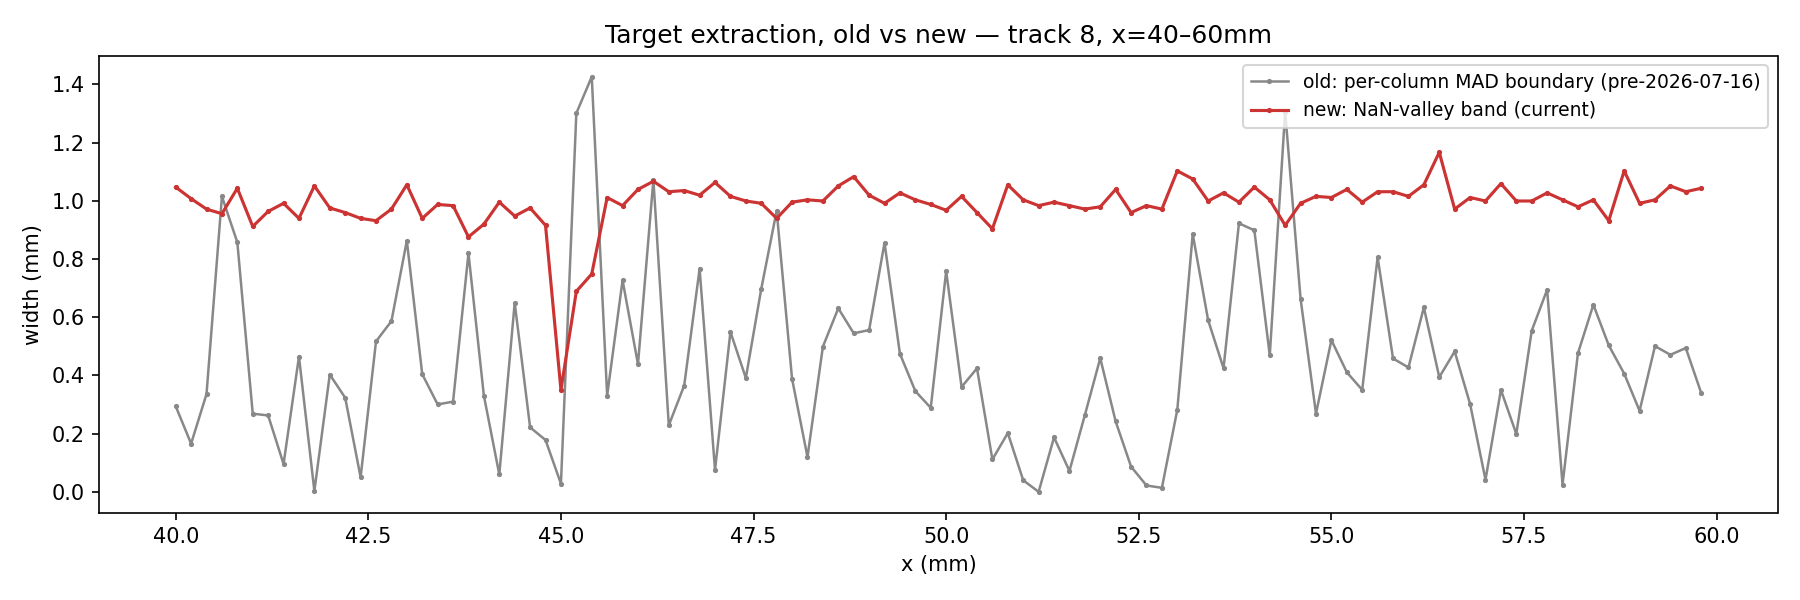
\includegraphics[width=\textwidth]{../results/report_figures/target_redefinition_before_after.png}
  \caption{TODO}
  \label{fig:target-redef}
\end{figure}

\subsection{Thermal imaging features}
TODO

\subsection{SEM imagery: substrate screening and a negative result}
TODO

\section{Methodology}

\subsection{Cross-validation protocol}
TODO

\subsection{Candidate models}
TODO

\begin{table}[h]
\centering
\begin{tabular}{lrrrr}
\toprule
Model & MAE (mm) & NLL & coverage$_{90}$ & t21 median (mm) \\
\midrule
constant & & & & \\
anchor GP & & & & \\
phys\_gp (inflated) & & & & \\
area1d & & & & \\
\textbf{linear3 [PRIMARY]} & & & & \\
full18 (negative control) & & & & \\
\bottomrule
\end{tabular}
\caption{TODO: verify against metrics.json files before submitting.}
\label{tab:model-comparison}
\end{table}

\begin{figure}[h]
  \centering
  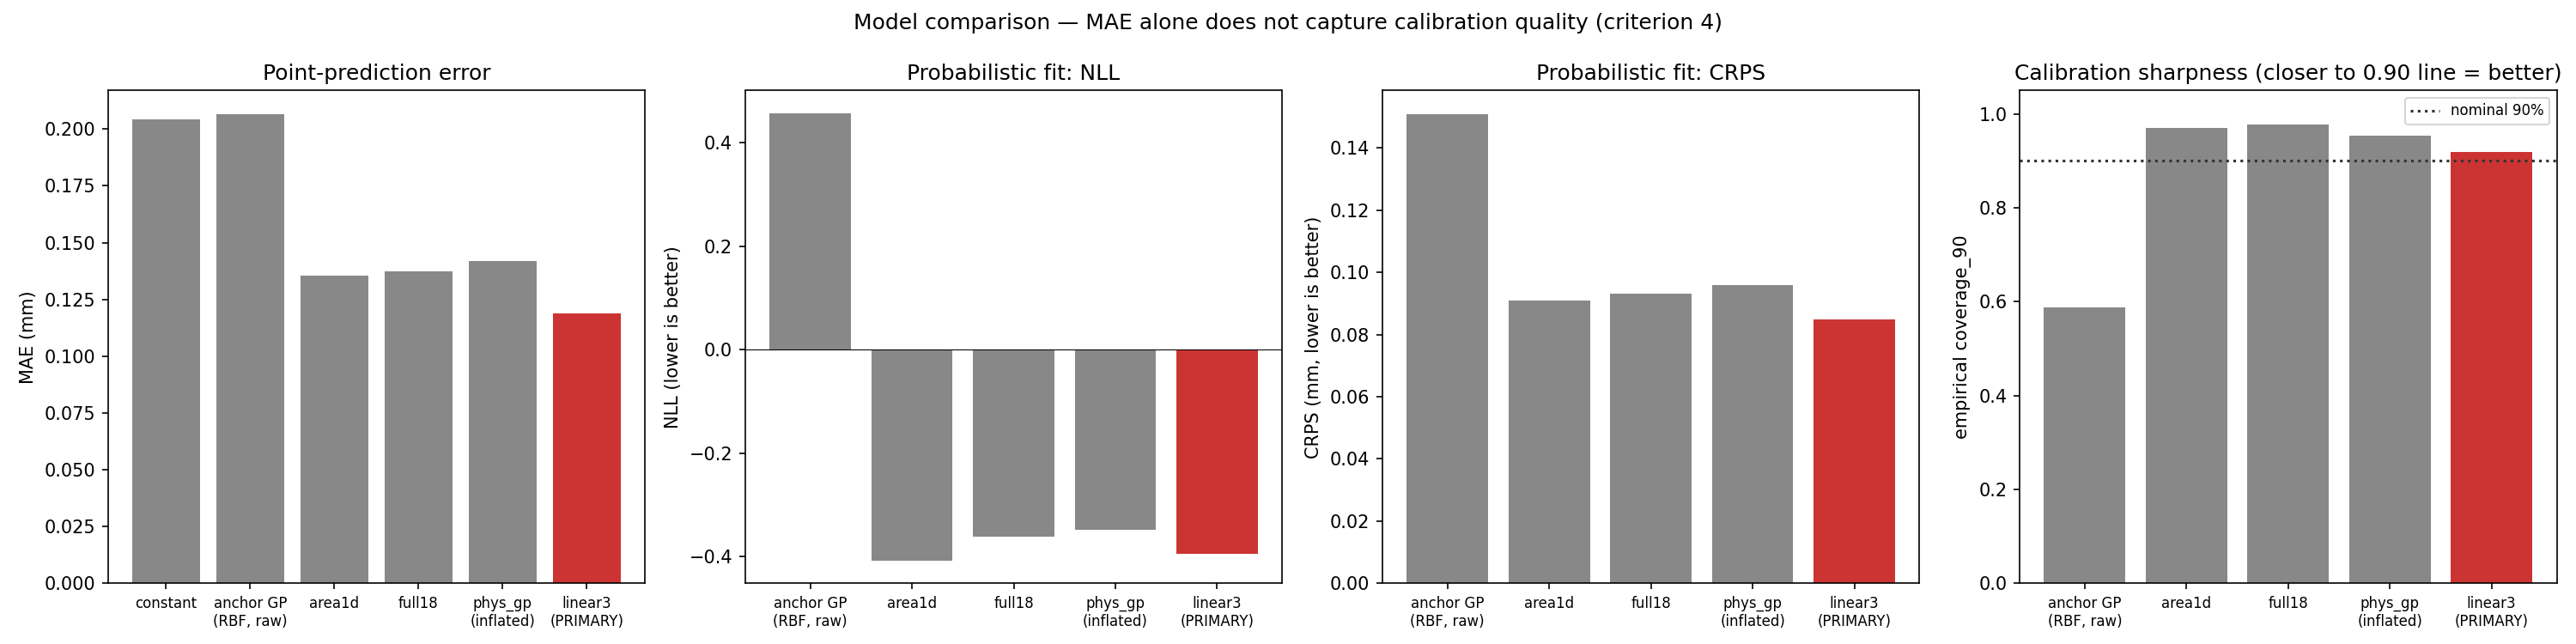
\includegraphics[width=\textwidth]{../results/report_figures/model_comparison_full.png}
  \caption{TODO}
  \label{fig:model-comparison}
\end{figure}

\subsection{Calibration: cross-fold variance inflation}
TODO

\begin{figure}[h]
  \centering
  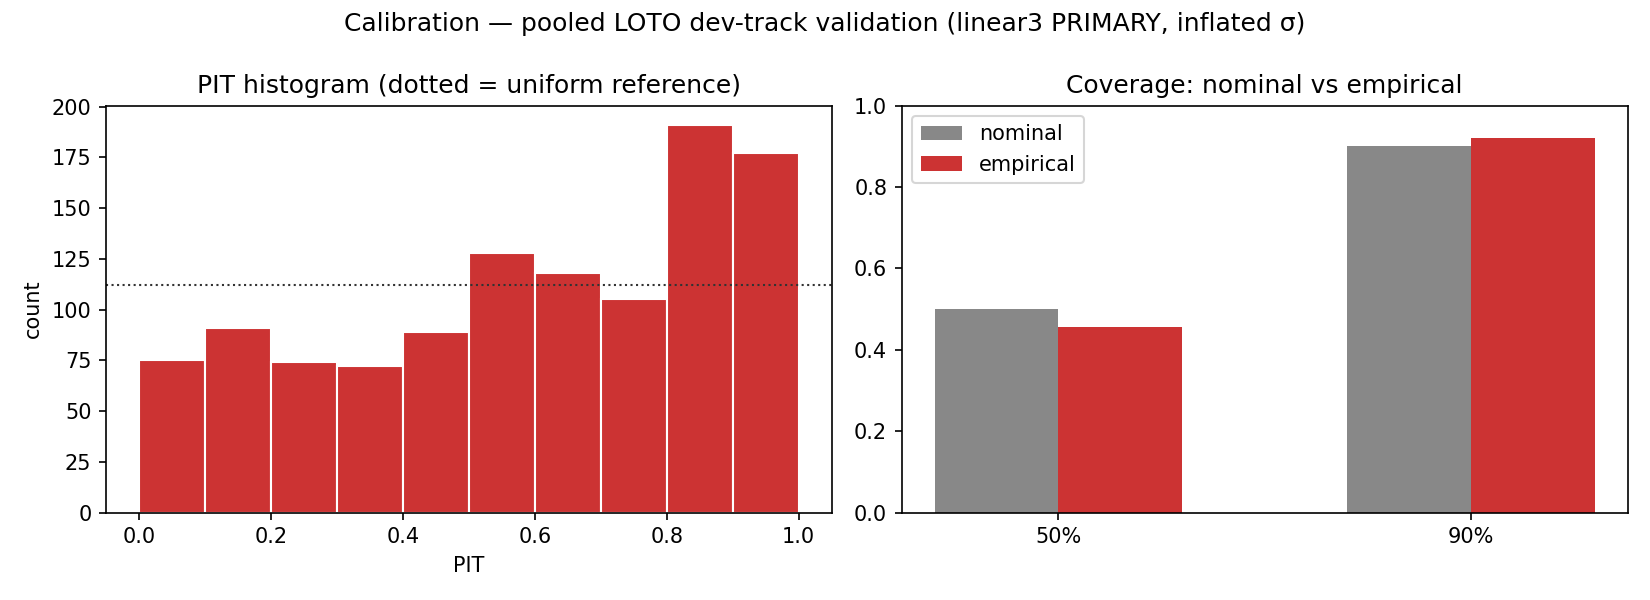
\includegraphics[width=0.8\textwidth]{../results/report_figures/calibration_diagnostics.png}
  \caption{TODO}
  \label{fig:calibration}
\end{figure}

\section{Results}

\subsection{LOTO width prediction}
\begin{figure}[h]
  \centering
  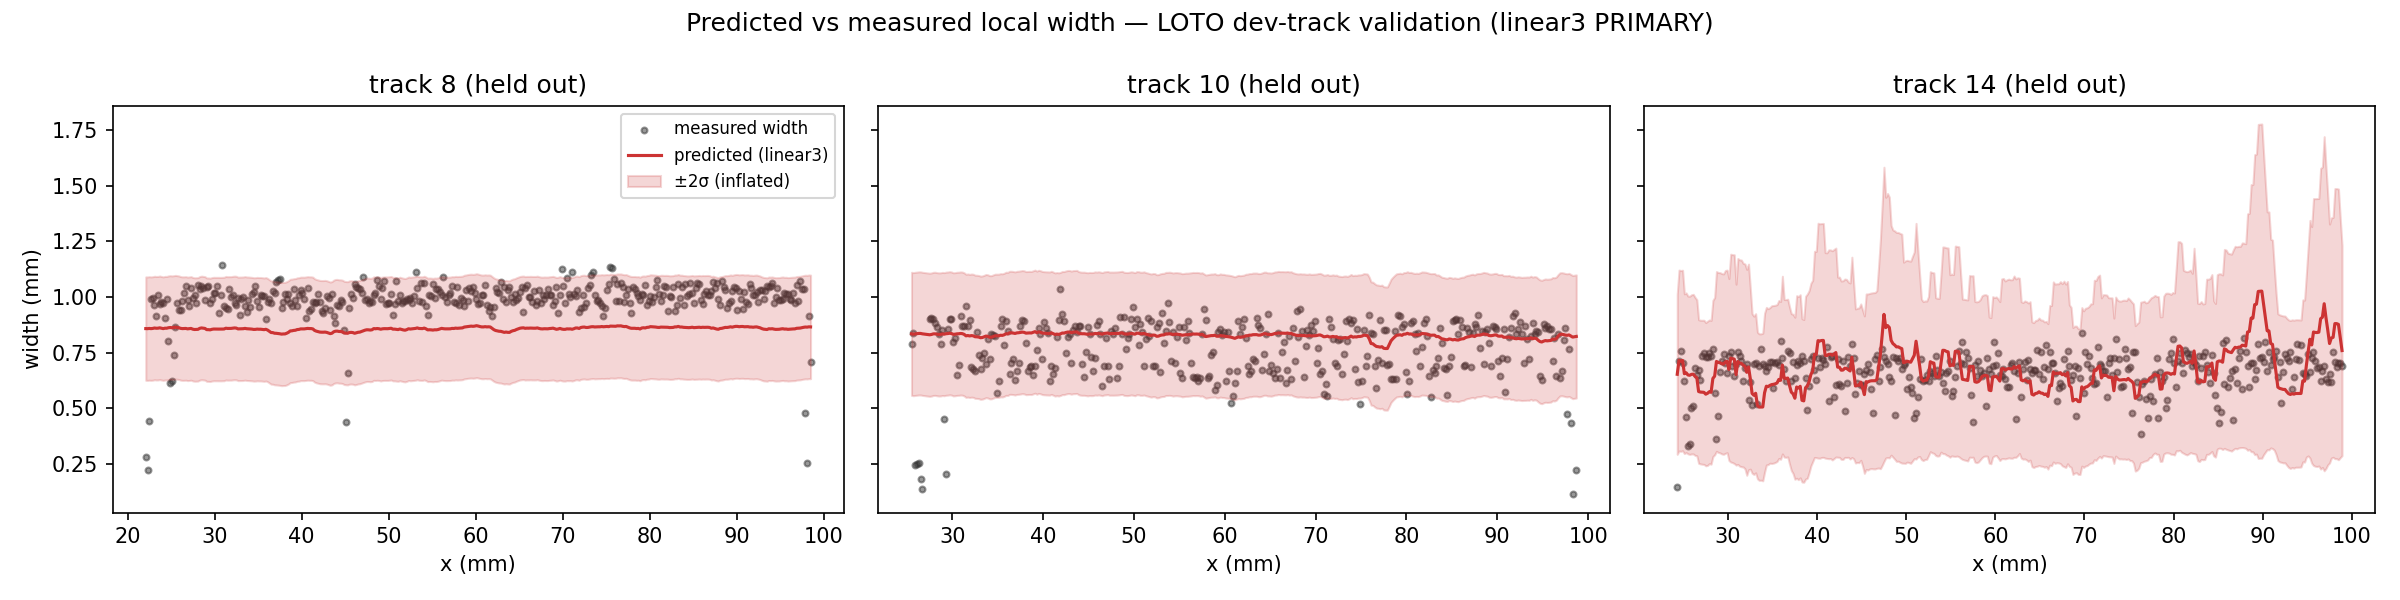
\includegraphics[width=\textwidth]{../results/report_figures/width_loto_comparison.png}
  \caption{TODO}
  \label{fig:width-loto}
\end{figure}

\subsection{Waviness as an additional output}
TODO

\begin{figure}[h]
  \centering
  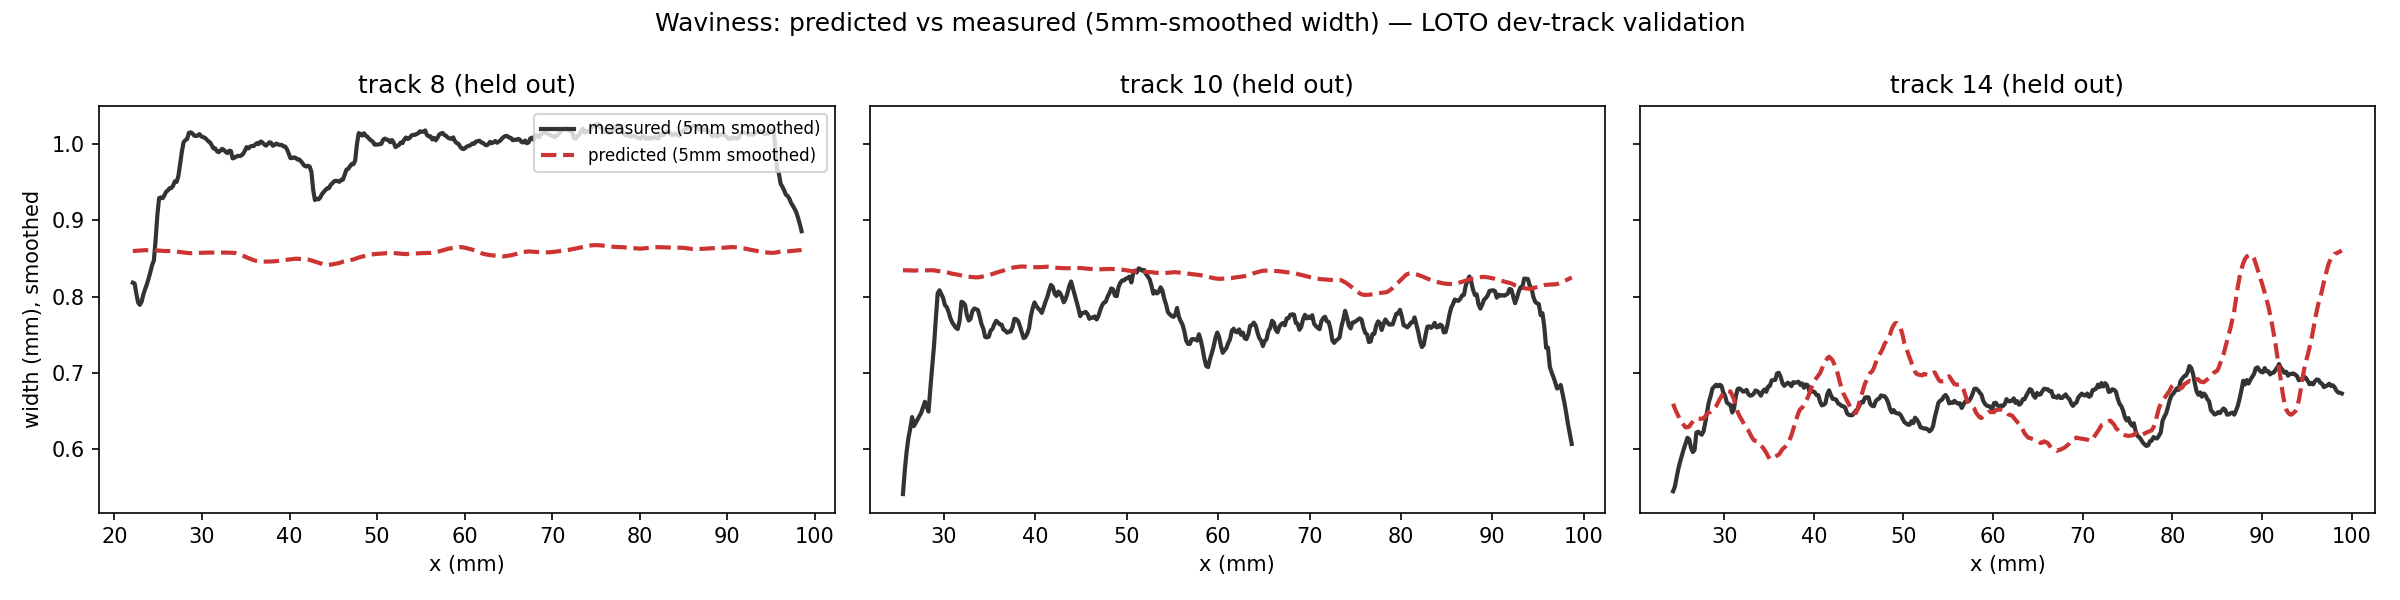
\includegraphics[width=\textwidth]{../results/report_figures/waviness_loto_comparison.png}
  \caption{TODO}
  \label{fig:waviness-loto}
\end{figure}

\subsection{Track-21 prediction and submission}
TODO

\begin{figure}[h]
  \centering
  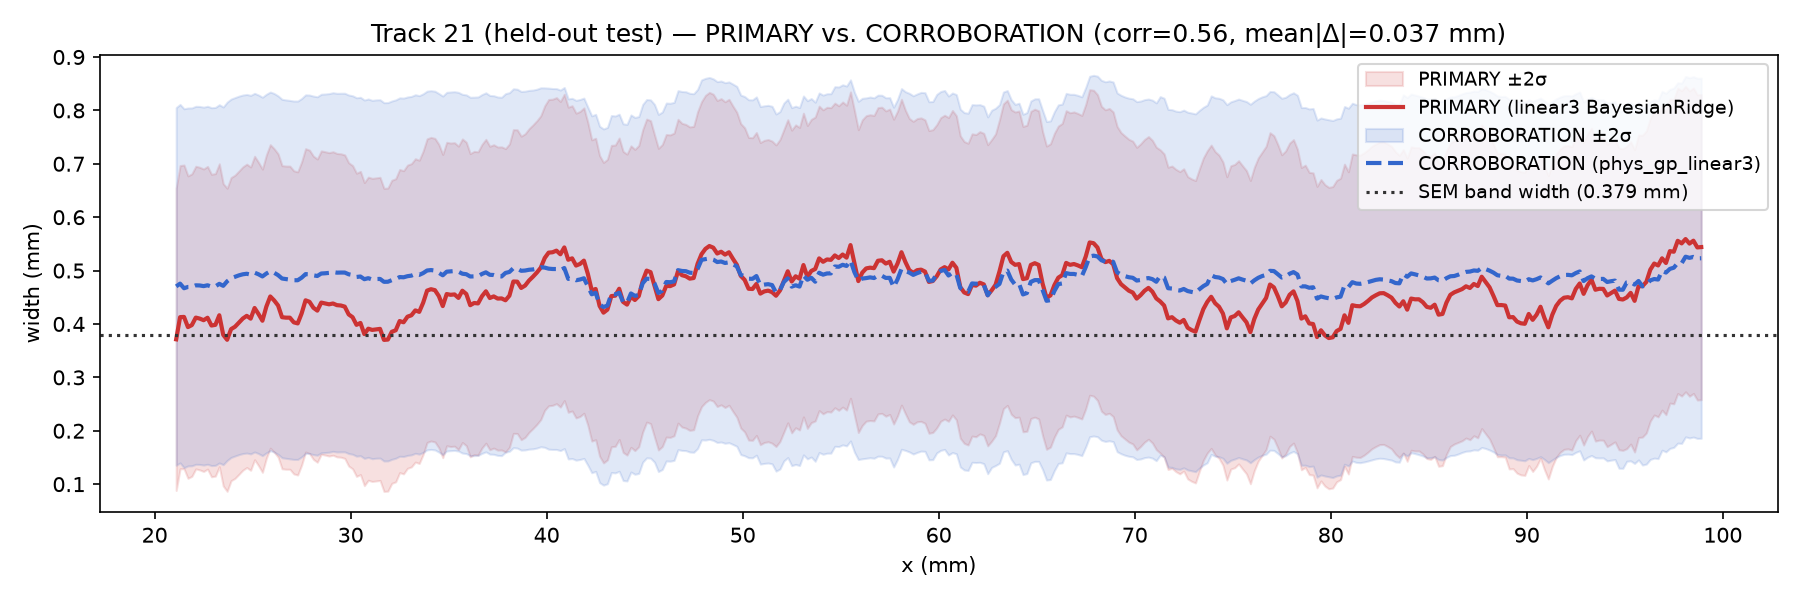
\includegraphics[width=\textwidth]{../results/report_figures/track21_prediction.png}
  \caption{TODO}
  \label{fig:t21-corroboration}
\end{figure}

\subsection{Width/SEM-band ratio: an honest open tension}
TODO

\section{Discussion and Limitations}

\subsection{Why not boundary/centerline}
TODO

\subsection{Criterion (2): spatial-variation fidelity, self-derived}
TODO

\subsection{Within-track noise floor and the PIT skew}
TODO

\subsection{Uncertainty submission format}
TODO

\section{Conclusion}
TODO

\appendix
\section{Reproducibility}
TODO

\end{document}
